\section{Auswertung}
\label{sec:Auswertung}



\subsection{Magnetfeldstärke}
Im ersten Schritt wird die Stärke des Magnetfelds in Abhängigkeit von der Sondenposition 
gemessen. Das Magnetfeld wird von einem Elektromagneten erzeugt. Die gemessenen Werte sind in \ref{tab:Tabelle 1}
Tabelle angegeben, in Abbildung \ref{fig: Abbildung 1} ist die magnetische Flussdichte gegen die Position der Sonde geplottet.

\begin{table}[h]
\centering
\begin{tabular}{|c|c|}
\hline   
\(z\)/mm & \(B\)/ \(mT\) \\
\hline
40 & 0.6 \\ 
50 & 1.1 \\ 
60 & 0.8 \\ 
70 & 0.3 \\ 
80 & 0.3 \\ 
90 & 0.3 \\
100 & 0.6 \\ 
105 & 0.9 \\
110 & 1.7 \\ 
115 & 5.0 \\
120 & 17.3 \\ 
125 & 56.9 \\ 
130 & 214 \\
135 & 394 \\
140 & 421 \\ 
145 & 414 \\
150 & 354 \\ 
55 & 134 \\ 
160 & 26 \\
165 & 6 \\ 
170 & 1.6 \\
\hline
\end{tabular}
\caption{Messwerte des Magnetfeldes $B$ bei verschiedenen Positionen $z$} 
\label{tab:Tabelle 1}
\end{table}

\begin{figure}
    \centering
    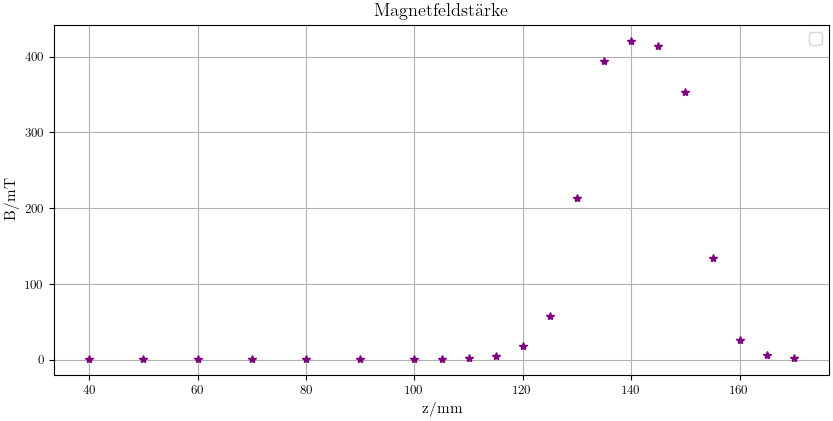
\includegraphics[width=\textwidth]{Bilder/Magnetfeld.png}
    \caption{Die Kraftflussdichte \(B(z)\)}
    \label{fig: Abbildung 1}
\end{figure}
Der maximal von uns gemessene Wert beträgt 421 \(mT\).

\subsection{Drehwinkel der Faraday-Rotation}
Für jede Probe wird die Messreihe zweimal durchgeführt, den Drehwinkel berechnet man nach :
\begin{equation}
    \theta_{nom}=\frac{\theta_1-\theta_2}{2}
\end{equation}    

Die folgenden drei Tabellen representieren die gemessenen Winkel, die normierten Winkel, sowie die Wellenlänge. Die Dotierung und die Dicke der Probe werden jeweils angegeben. 


\begin{table}[h]
\centering
\caption{Dotierung: \( N = 1.2\cdot10^{18} \, \text{cm}^{-3} \)
Dicke der Probe: 1.36 mm}
\begin{tabular}{|c|c|c|c|c|}
\hline    
$\theta_1$ / Grad & $\theta_2$ / Grad & $\theta_{nom}$ /Grad & $\theta_{nom}$ / Rad & $\lambda$ / $\mu$m \\
72.91 & 82.66 & 9.75 & 0.170 & 1.06 \\
73.11 & 80.83 & 7.72 & 0.134 & 1.29 \\
73.71 & 80.83 & 7.12 & 0.124 & 1.45 \\ 
72.58 & 78.78 & 6.2 & 0.108 & 1.72 \\ 
68.2 & 73.85 & 5.65 & 0.098 & 1.96 \\
64.28 & 70.93 & 6.65 & 0.116 & 2.156 \\
40.33 & 48.16 & 7.83 & 0.136 &2.32 \\
30.0 & 37.0 & 2.51 & 7 & 0.122 \\
59.3 & 68.01 &8.71 & 0.152 & 2.65 \\
\hline
\end{tabular}
\label{tab:winkel_wellenlaenge1} 
\end{table}



\begin{table}[h] 
\centering 
\caption{Dotierung: \( N = 2.8\cdot10^{18} \, \text{cm}^{-3} \)
Dicke der Probe: 1.296 mm}
\begin{tabular}{|c|c|c|c|c|} 
\hline
$\theta_1$ / Grad & $\theta_2$ / Grad & $\theta_{nom}$ / Grad & $\theta_{nom}$ / Rad & $\lambda$ / $\mu$m \\
\hline 
71.76 & 82.83 & 5.535 & 0.0966 & 1.06 \\
72.71 & 80.75 & 4.02 & 0.0702 & 1.29 \\
72.58 & 81.28 & 4.35 & 0.0759 & 1.45 \\
70.33 & 79.51 & 4.59 & 0.0801 & 1.72 \\
66.83 & 77.38 & 5.275 & 0.0920 & 1.96 \\
62.0 & 73.38 & 5.69 & 0.0994 & 2.156 \\
39.01 & 51.46 & 6.225 & 0.1086 & 2.34 \\ 
26.56 & 41.9 & 7.67 & 0.1339 & 2.51 \\
58.73 & 72.63 & 6.95 & 0.1213 & 2.65 \\  
\hline 
\end{tabular} 
\label{tab:winkel_wellenlaenge2} 
\end{table}

Dicke der Probe: 1.296 mm, undotiert

\begin{table}[h] 
\centering 
\caption{Dicke der Probe: 1.296 mm, undotiert}
\begin{tabular}{|c|c|c|c|c|} 
\hline
$\theta_1$ / Grad & $\theta_2$ / Grad & $\theta_{nom}$ / Grad & $\theta_{nom}$ / Rad & $\lambda$ / $\mu$m \\ 
\hline 
66.28 & 89.33 & 11.525 & 0.2012 & 1.06 \\
70.4 & 85.0 & 7.3 & 0.1274 & 1.29 \\
73.25 & 84.7 & 5.725 & 0.0999 & 1.45 \\
41.0 & 80.76 & 19.88 & 0.3468 & 1.72 \\
68.83 & 76.3 & 3.735 & 0.0652 & 1.96 \\
65.91 & 70.35 & 2.22 & 0.0387 & 2.156 \\
42.71 & 46.38 & 1.835 & 0.0320 & 2.34 \\
29.71 & 32.25 & 1.27 & 0.0222 & 2.51 \\
59.33 & 65.18 & 2.925 & 0.0510 & 2.65 \\ 
\hline 
\end{tabular} 
\label{tab:winkel_wellenlaenge3} 
\end{table}
\FloatBarrier

Zur veranschaulichung der Messergebnisse werden die normierten Winkel in \ref{fig:2} gegen die Wellenlänge geplottet
\begin{figure}
    \centering
    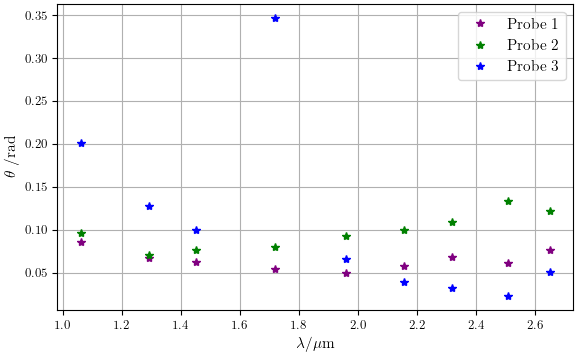
\includegraphics[width=\textwidth]{Bilder/Probe1-3.png}
    \caption{Die normierten Drehwinkel der drei Proben}
    \label{fig:2}
\end{figure}
 
Im nächsten Schritt wird die Differenz der Faraday-Rotation zwischen dotierter und undotierter Probe
gebildet, um den Effekt der Leitungselektronen genau zu untersuchen. Die berechneten Drehwinkel sind in 
Abbildung \ref{fig:differenzen}  gegen $\lambda^2$ geplottet.

\begin{figure}
    \centering
    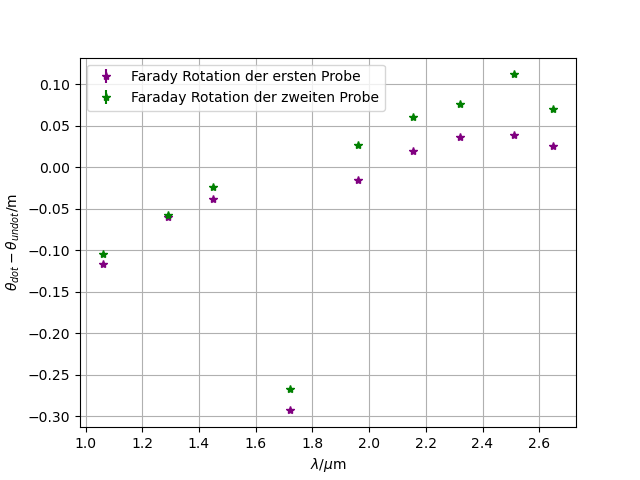
\includegraphics[width=\textwidth]{Bilder/differenzen.png}
    \caption{Die Differenzen der Drehwinkel von den dotierten und der undotierten Probe}
    \label{fig:differenzen}
\end{figure}


\subsection{Bestimmung der Effektiven Masse}
Die Effektive Masse beschreibt, wie Elektronen auf das angelegte Magnetfeld reagieren, was die Drehung der
polarisationsebene des durch das Material gehenden Lichts beeinflusst. Die Effektive Masse kann je nach Material 
und seiner elektronischen Bandstruktur variieren. Sie wird durch die Differenzen der Drehwinkel $\theta_{nom}$ 
der dotierten und der undotierten Probe berechnet. Dazu wird eine eine lineare Ausgleichsrechnung mit Python 
durchgeführt die die Form:
\begin{equation}
g(x)=mx+b
\label{eq:lineareform}
\end{equation}
hat.

\begin{figure}
    \centering
    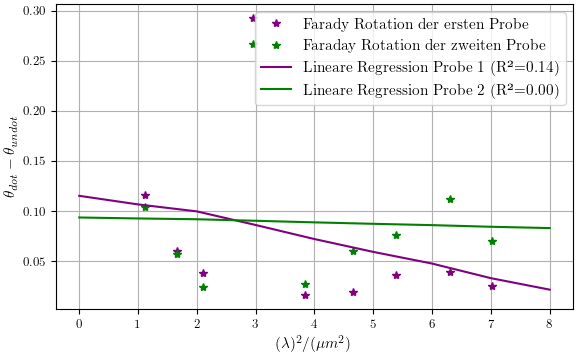
\includegraphics[width=\textwidth]{Bilder/lineareregression.png}
    \caption{Die Differenzen der Drehwinkel von den dotierten und der undotierten Probe inklusive linearer regression}
    \label{fig:regression}
\end{figure}

Die Effektive Masse berechnet sich nach:
\begin{equation}
    \theta_{frei}=\frac{(e_0)^3 \lambda^2 NB}{8 \pi\epsilon_0 c^3 (m^*)^2 n}
\label{eq:masse}
\end{equation}

Aus der linearen Regression wird der Proportionalitätsfaktor $m$  bestimmt.
Dabei entspricht g(x) der gemessenen Faraday-Rotation $\theta_{frei}$ und x
entspricht dem quadrat der Wellenlänge $\lambda^2$.

Setzt man die lineare Form der regression in \eqref{eq:masse} ein erhält man eine Gleichung der Form :
\begin{equation}
    \theta_{frei}=k\lambda^2
\end{equation}
Wobei $k$ der proportionalitätsfaktor ist und $m$ aus der linearen Regression entspricht:
\begin{equation}
    k=\frac{(e_0)^3NB}{8\pi^2\epsilon_0 c^3(m^*)^2 n}
\end{equation}
Löst man nach $m^*$ auf, setzt $k=m$ und zieht die Wurzel so ergibt sich für die Effektive Masse 
folgende Beziehung:
\begin{equation}
    m^*=\sqrt{\frac{(e_0)^3NB}{8\pi^2 \epsilon_0 c^3 m n}}
\end{equation}   
Dabei ist $e_0=1.603\cdot10^{-19}C$ die Elementarladung, $\epsilon_0=8.85\cdot10^{-12}F/m$ die Dielektrizitätskonstante des Materials,
$c=3\cdot10^8 m/s$ die Lichtgeschwindigkeit, $n$=3.5 der brechungsindex für GaAs und $B= 421 mT$ die maximale Kraftflussdichte.
$N$ ist die Dotierungsschicht, die für die beiden Proben verschieden dick ist.
$m$ wird mit Phyton und scipy bestimmt.

\begin{itemize} 
    \item Probe 1: \(N = 1.2 \cdot 10^{18} \, \text{cm}^{-3}\), Proportionalitätsfaktor \(m_1 = 0.01588407903456512\)
Damit ergibt sich die effektive Masse:
\begin{equation} m^*_1 = 3.8869115 \cdot 10^{-28} \, \text{kg}
\end{equation}
\item Probe 2: \(N = 2.8 \cdot 10^{18} \, \text{cm}^{-3}\), Proportionalitätsfaktor \(m_2 = 0.0017916113751336978\)
Damit ergibt sich die effektive Masse:
\begin{equation} m^*_2 = 1.767877 \cdot 10^{-27} \, \text{kg} 
\end{equation} 
\end{itemize}

    
    














